% summary_results.tex — JMIR-style results section
% Metrics: Modal MAE (lower = better) and EAD (lower = better).
% Question split: Perception = Q1, Q10 per DS; Information = Q2--Q9 per DS.
% Subgroups: Edu-Low/High, Male/Female, OutLow/High, ERLow (7 total).
% Frequency classification: weekly|monthly = high; yearly|never = low.

\subsection{Subgroup-Level Alignment With Human Responses}

Tables~\ref{tab:perc-distance-alignment}--\ref{tab:info-expdist-alignment} present
distance-based alignment between each large language model (LLM) subgroup and the
matched human subgroup (eg, LLM Edu-Low vs Human Edu-Low). Two complementary metrics
are reported. Modal mean absolute error (MAE) measures the ordinal distance between
the most frequently chosen answer of the LLM subgroup and that of the corresponding
human subgroup; expected absolute distance (EAD) integrates over the full marginal
response distributions and captures distributional calibration beyond the mode.
Lower values indicate better alignment; the theoretical maximum is 4 under the
ordinal coding A\,$=$\,0, B\,$=$\,1, C\,$=$\,2, D\,$=$\,3, E\,$=$\,4.

Each table includes a \emph{Human (split-half)} baseline row: human respondents
within each subgroup were randomly split into 2 halves and the same metric was
computed between halves, averaged over 200 bootstrap resamples. This baseline
quantifies the natural noise floor attributable to within-subgroup disagreement
and finite sample size.

% ---------- Table 1: Perception Modal MAE ----------
\begin{table}[htbp]
\centering
\scriptsize
\setlength{\tabcolsep}{3.5pt}
\caption{Distance-based alignment for Perception-based questions (Q1 and Q10 per DS, $n{=}8$): Modal MAE between each LLM subgroup and the matched human subgroup. Lower is better.}
\label{tab:perc-distance-alignment}
\begin{tabular}{lcccccccc}
\toprule
\textbf{Model}
& \multicolumn{2}{c}{\textbf{Education}}
& \multicolumn{2}{c}{\textbf{Sex}}
& \multicolumn{2}{c}{\textbf{Outpatient}}
& \textbf{ED Visits}
& \textbf{Max} \\
\cmidrule(lr){2-3}\cmidrule(lr){4-5}\cmidrule(lr){6-7}
& Low & High & Male & Female & Low & High & Low & \\
\midrule
Sonnet 4.5 & \textbf{1.62} & 0.75 & 0.75 & 0.62 & 0.75 & 0.88 & 0.62 & 4 \\
Opus 4.6 & 1.38 & 1.25 & 1.12 & 1.12 & 1.00 & 0.38 & 1.00 & 4 \\
GPT-5.2 & 1.12 & 1.25 & 0.88 & 0.50 & 0.75 & 1.00 & 0.88 & 4 \\
GPT-4.1 & 1.38 & 1.12 & \textbf{1.25} & 0.62 & 0.88 & 1.12 & 1.12 & 4 \\
\midrule
\textit{Human (split-half)} & 0.39 & 0.64 & 0.27 & 0.59 & 0.47 & 0.82 & 0.36 & 4 \\
\bottomrule
\end{tabular}
\end{table}

% ---------- Table 2: Perception EAD ----------
\begin{table}[htbp]
\centering
\scriptsize
\setlength{\tabcolsep}{3.5pt}
\caption{Distribution-level alignment for Perception-based questions: expected absolute ordinal distance $\mathbb{E}[|\mathrm{ord}(\hat{Y}_{\mathrm{LLM}})-\mathrm{ord}(Y_{\mathrm{Human}})|]$ over matched subgroups.}
\label{tab:perc-expdist-alignment}
\begin{tabular}{lcccccccc}
\toprule
\textbf{Model}
& \multicolumn{2}{c}{\textbf{Education}}
& \multicolumn{2}{c}{\textbf{Sex}}
& \multicolumn{2}{c}{\textbf{Outpatient}}
& \textbf{ED Visits}
& \textbf{Max} \\
\cmidrule(lr){2-3}\cmidrule(lr){4-5}\cmidrule(lr){6-7}
& Low & High & Male & Female & Low & High & Low & \\
\midrule
Sonnet 4.5 & \textbf{1.30} & 0.85 & 0.97 & 1.02 & 0.98 & 1.08 & 0.97 & 4 \\
Opus 4.6 & 1.11 & 1.23 & 1.03 & 1.05 & 1.04 & 1.02 & 1.03 & 4 \\
GPT-5.2 & 1.03 & 1.08 & 0.92 & 0.98 & 0.96 & 0.93 & 0.95 & 4 \\
GPT-4.1 & 1.11 & 1.18 & 0.99 & 1.02 & 1.01 & 0.99 & 1.01 & 4 \\
\midrule
\textit{Human (split-half)} & 0.91 & 0.91 & 0.83 & 0.96 & 0.92 & 0.88 & 0.94 & 4 \\
\bottomrule
\end{tabular}
\end{table}

% ---------- Table 3: Information Modal MAE ----------
\begin{table}[htbp]
\centering
\scriptsize
\setlength{\tabcolsep}{3.5pt}
\caption{Distance-based alignment for Information-based questions (Q2--Q9 per DS, $n{=}32$): Modal MAE between each LLM subgroup and the matched human subgroup.}
\label{tab:info-distance-alignment}
\begin{tabular}{lcccccccc}
\toprule
\textbf{Model}
& \multicolumn{2}{c}{\textbf{Education}}
& \multicolumn{2}{c}{\textbf{Sex}}
& \multicolumn{2}{c}{\textbf{Outpatient}}
& \textbf{ED Visits}
& \textbf{Max} \\
\cmidrule(lr){2-3}\cmidrule(lr){4-5}\cmidrule(lr){6-7}
& Low & High & Male & Female & Low & High & Low & \\
\midrule
Sonnet 4.5 & 1.20 & 1.06 & \textbf{1.21} & 1.00 & 1.25 & 1.00 & 1.14 & 4 \\
Opus 4.6 & 0.72 & 0.68 & 0.68 & 0.57 & 0.86 & 0.57 & 0.69 & 4 \\
GPT-5.2 & \textbf{0.88} & 0.65 & 0.71 & 0.68 & 0.86 & 0.71 & 0.62 & 4 \\
GPT-4.1 & 1.00 & 0.90 & 0.75 & 0.71 & 0.79 & 0.79 & 0.76 & 4 \\
\midrule
\textit{Human (split-half)} & 0.55 & 0.32 & 0.52 & 0.37 & 0.40 & 0.41 & 0.35 & 4 \\
\bottomrule
\end{tabular}
\end{table}

% ---------- Table 4: Information EAD ----------
\begin{table}[htbp]
\centering
\scriptsize
\setlength{\tabcolsep}{3.5pt}
\caption{Distribution-level alignment for Information-based questions: expected absolute ordinal distance over matched subgroups.}
\label{tab:info-expdist-alignment}
\begin{tabular}{lcccccccc}
\toprule
\textbf{Model}
& \multicolumn{2}{c}{\textbf{Education}}
& \multicolumn{2}{c}{\textbf{Sex}}
& \multicolumn{2}{c}{\textbf{Outpatient}}
& \textbf{ED Visits}
& \textbf{Max} \\
\cmidrule(lr){2-3}\cmidrule(lr){4-5}\cmidrule(lr){6-7}
& Low & High & Male & Female & Low & High & Low & \\
\midrule
Sonnet 4.5 & 0.95 & 1.01 & \textbf{1.05} & 1.00 & 1.11 & 0.98 & 1.07 & 4 \\
Opus 4.6 & 0.69 & 0.76 & 0.81 & 0.75 & 0.86 & 0.74 & 0.81 & 4 \\
GPT-5.2 & 0.80 & 0.78 & 0.86 & 0.78 & 0.89 & 0.82 & 0.86 & 4 \\
GPT-4.1 & 0.85 & 0.89 & 0.93 & 0.89 & 0.96 & 0.93 & 0.96 & 4 \\
\midrule
\textit{Human (split-half)} & 0.75 & 0.59 & 0.70 & 0.60 & 0.66 & 0.66 & 0.67 & 4 \\
\bottomrule
\end{tabular}
\end{table}

\subsection{Education and Sex Equity Gaps}

To quantify how equitably each model simulates different patient populations, we computed the absolute gap between paired subgroups (Education: Low$-$High;
Sex: Male$-$Female) for all 4 metrics. A positive education gap indicates worse alignment for the low-education subgroup; a positive sex gap indicates
worse alignment for the male subgroup. Results are summarized in Tables~\ref{tab:edu-gap} and~\ref{tab:sex-gap}. The largest observed gap in each
metric is highlighted in bold.

% ---------- Table 5: Education Equity Gap ----------
\begin{table}[htbp]
\centering
\scriptsize
\setlength{\tabcolsep}{4.5pt}
\caption{Education equity gap (Edu-Low minus Edu-High). Positive values indicate
poorer alignment for the low-education subgroup. Bold marks the largest absolute
gap per metric.}
\label{tab:edu-gap}
\begin{tabular}{lrrrr}
\toprule
\textbf{Model}
& \textbf{Modal MAE} & \textbf{Modal MAE} & \textbf{EAD} & \textbf{EAD} \\
& \textbf{(Perception)} & \textbf{(Information)} & \textbf{(Perception)} & \textbf{(Information)} \\
\midrule
Sonnet 4.5 & \textbf{+0.875} & +0.135            & \textbf{+0.455}  & $-$0.055 \\
Opus 4.6   & +0.125           & +0.043            & $-$0.123         & \textbf{$-$0.067} \\
GPT-5.2    & $-$0.125         & \textbf{+0.235}   & $-$0.052         & +0.018 \\
GPT-4.1    & +0.250           & +0.097            & $-$0.068         & $-$0.033 \\
\bottomrule
\end{tabular}
\end{table}

% ---------- Table 6: Sex Equity Gap ----------
\begin{table}[htbp]
\centering
\scriptsize
\setlength{\tabcolsep}{4.5pt}
\caption{Sex equity gap (Male minus Female). Positive values indicate poorer alignment
for the male subgroup. Bold marks the largest absolute gap per metric.}
\label{tab:sex-gap}
\begin{tabular}{lrrrr}
\toprule
\textbf{Model}
& \textbf{Modal MAE} & \textbf{Modal MAE} & \textbf{EAD} & \textbf{EAD} \\
& \textbf{(Perception)} & \textbf{(Information)} & \textbf{(Perception)} & \textbf{(Information)} \\
\midrule
Sonnet 4.5 & +0.125           & \textbf{+0.214}   & $-$0.053          & +0.051 \\
Opus 4.6   & 0.000            & +0.107             & $-$0.017          & +0.063 \\
GPT-5.2    & +0.375           & +0.036             & \textbf{$-$0.061} & \textbf{+0.079} \\
GPT-4.1    & \textbf{+0.625}  & +0.036             & $-$0.024          & +0.042 \\
\bottomrule
\end{tabular}
\end{table}

\subsubsection{Education Gap}

The most prominent finding was the large education gap exhibited by Sonnet~4.5:
its modal MAE for the low-education subgroup on perception questions was 1.62,
compared with 0.75 for the high-education subgroup---a gap of \textbf{+0.875}
(Table~\ref{tab:edu-gap}), the largest observed across all model-metric
combinations. The corresponding distributional metric (EAD) confirmed this
disparity (gap$=$+0.455). These results indicate that Sonnet~4.5 defaults
to a response pattern more representative of highly educated individuals and
fails to capture how patients with lower health literacy perceive discharge
summaries.

By contrast, Opus~4.6 demonstrated the most equitable education-level performance:
its perception modal MAE gap was only +0.125, and its EAD gap slightly favored
the low-education subgroup ($-$0.123). GPT-5.2 was the only model that achieved
better modal alignment for the low-education group on perception questions
(gap$=$$-$0.125); however, it showed the largest education gap on
information-based questions (+0.235).

\subsubsection{Sex Gap}

The largest sex gap on perception modal MAE was observed for GPT-4.1
(\textbf{+0.625}; Table~\ref{tab:sex-gap}), driven by a male-subgroup
score of 1.25 versus a female-subgroup score of 0.62. This gap
was attributable to mode flips rather than broad distributional
mismatch, as the EAD gap for the same model was only $-$0.024.

For information-based questions, Sonnet~4.5 exhibited the largest sex gap
on modal MAE (+0.214; male$=$1.21, female$=$1.00).
Opus~4.6 was the most sex-equitable model overall: its perception modal MAE
was identical across sexes (1.12 vs 1.12; gap$=$0.000), and its
information EAD gap was modest (+0.063).

Across all models, EAD sex gaps were uniformly small ($\le$0.079),
suggesting that the sex-based differences visible in modal MAE
largely reflect mode-switching sensitivity rather than systematic
distributional bias.


\subsection{Effect of Discharge Summary Type on Education Gap}

Given that Sonnet~4.5 exhibited the largest education equity gap overall, we
examined how discharge summary (DS) characteristics modulate this gap. The 4
discharge summaries varied along 2 dimensions---length (short vs long) and
medical complexity (simple vs difficult):

\begin{itemize}\itemsep0pt
\item DS1: Short \& Difficult
\item DS2: Long \& Simple
\item DS3: Long \& Difficult
\item DS4: Short \& Simple
\end{itemize}

Table~\ref{tab:ds-edu-gap} reports per-DS alignment scores for Sonnet~4.5,
stratified by education level, for both perception- and information-based
questions.

% ---------- Table 7: Per-DS Education Gap (Sonnet 4.5) ----------
\begin{table}[htbp]
\centering
\scriptsize
\setlength{\tabcolsep}{3.5pt}
\caption{Per-DS education-level alignment for Sonnet~4.5. For each discharge
summary type, modal MAE and EAD are reported for the Edu-Low and Edu-High
subgroups, along with the education gap ($\Delta$\,$=$\,Low$-$High). Bold
marks the largest gap per metric block. Perception: $n$=2 questions per DS;
Information: $n$=8 questions per DS.}
\label{tab:ds-edu-gap}
\begin{tabular}{llrrrrrrr}
\toprule
 & & \multicolumn{3}{c}{\textbf{Modal MAE}} & \multicolumn{3}{c}{\textbf{EAD}} \\
\cmidrule(lr){3-5}\cmidrule(lr){6-8}
\textbf{Type} & \textbf{DS}
& \textbf{Edu-Low} & \textbf{Edu-High} & $\boldsymbol{\Delta}$
& \textbf{Edu-Low} & \textbf{Edu-High} & $\boldsymbol{\Delta}$ \\
\midrule
Perception
& DS1: Short+Difficult & 1.50 & 0.00 & \textbf{+1.50} & 1.20 & 0.86 & +0.35 \\
& DS2: Long+Simple     & 1.50 & 0.50 & +1.00           & 1.17 & 0.79 & +0.38 \\
& DS3: Long+Difficult  & 1.50 & 1.00 & +0.50           & 1.32 & 0.76 & \textbf{+0.56} \\
& DS4: Short+Simple    & 2.00 & 1.50 & +0.50           & 1.52 & 0.99 & +0.54 \\
\cmidrule(lr){2-8}
& Overall              & 1.62 & 0.75 & +0.88           & 1.30 & 0.85 & +0.46 \\
\midrule
Information
& DS1: Short+Difficult & 0.25 & 0.75 & $-$0.50         & 0.24 & 0.79 & \textbf{$-$0.55} \\
& DS2: Long+Simple     & 1.43 & 1.00 & \textbf{+0.43}  & 1.29 & 1.10 & +0.19 \\
& DS3: Long+Difficult  & 1.29 & 1.38 & $-$0.09         & 1.05 & 1.03 & +0.01 \\
& DS4: Short+Simple    & 1.43 & 1.12 & +0.30           & 1.23 & 1.10 & +0.13 \\
\cmidrule(lr){2-8}
& Overall              & 1.20 & 1.06 & +0.14           & 0.95 & 1.01 & $-$0.06 \\
\bottomrule
\end{tabular}
\end{table}

\subsubsection{Perception Questions}

The education gap on perception questions was strongly modulated by DS type.
The largest gap occurred on \textbf{DS1 (Short \& Difficult)}: the model achieved
a modal MAE of 0.00 for Edu-High (ie, perfect modal agreement with highly educated
humans) but 1.50 for Edu-Low, yielding a gap of \textbf{+1.50}---the single largest
cell-level disparity in the entire analysis. DS2 (Long \& Simple) showed the
second-largest gap (+1.00). DS3 and DS4 had more moderate perception gaps (+0.50
each), though absolute Edu-Low scores remained high (1.50--2.00).

Per-question inspection revealed the mechanism: for low-education personas, Sonnet~4.5
consistently selected ``B'' or ``C'' for Q1 (overall clarity) and ``D'' for Q10
(confidence/comfort), regardless of DS type. Human Edu-Low respondents, however,
selected ``A'' (very clear/very confident) for Q1 in 3 of 4 discharge summaries
and ``B'' for Q10 across all 4. The model appears to assume that
low-education patients perceive discharge summaries as less clear and feel less
confident---an assumption not supported by the human data.

For high-education personas, the model's selections (predominantly ``B'') closely
matched human modes, explaining the near-zero gap on DS1.

\subsubsection{Information Questions}

On information-based questions, the education gap pattern reversed for DS1:
the Edu-Low subgroup aligned \textit{better} than Edu-High ($\Delta$\,$=$\,$-$0.50
for modal MAE; $-$0.55 for EAD). This suggests that the factual content of
the short, difficult discharge summary was captured differently by the model's
education-conditioned personas, with the low-education persona unexpectedly
producing more human-like factual answers.

DS2 (Long \& Simple) showed the largest positive information gap (+0.43),
indicating that longer, simpler documents amplified the model's tendency to
generate different information-extraction patterns for low- vs high-education
personas in a direction that diverged from actual human behavior.

\subsubsection{Interaction Between Length and Complexity}

Two patterns emerged from the DS-level analysis:

\begin{enumerate}\itemsep2pt
\item \textbf{Medical complexity amplifies the perception gap when documents are
  short.} DS1 (Short \& Difficult) produced the largest perception gap (+1.50),
  whereas DS4 (Short \& Simple) produced a smaller gap (+0.50). When a discharge
  summary is both brief and medically complex, the model's education-conditioned
  perception diverges most from human behavior---possibly because the model
  over-indexes on complexity as a cue that low-education patients would struggle,
  while actual low-education respondents did not report substantially lower clarity.

\item \textbf{Document length amplifies the information gap.} DS2 (Long \& Simple)
  had the largest positive information gap (+0.43), compared with DS1 (Short \&
  Difficult) where the gap reversed ($-$0.50). Longer documents provide more
  factual content to extract, and the model's persona conditioning appears to
  introduce education-dependent biases in how that content is processed---biases
  that do not reflect actual human variation.
\end{enumerate}

% ---------- Figure 1: Dumbbell chart ----------
\begin{figure}[htbp]
\centering
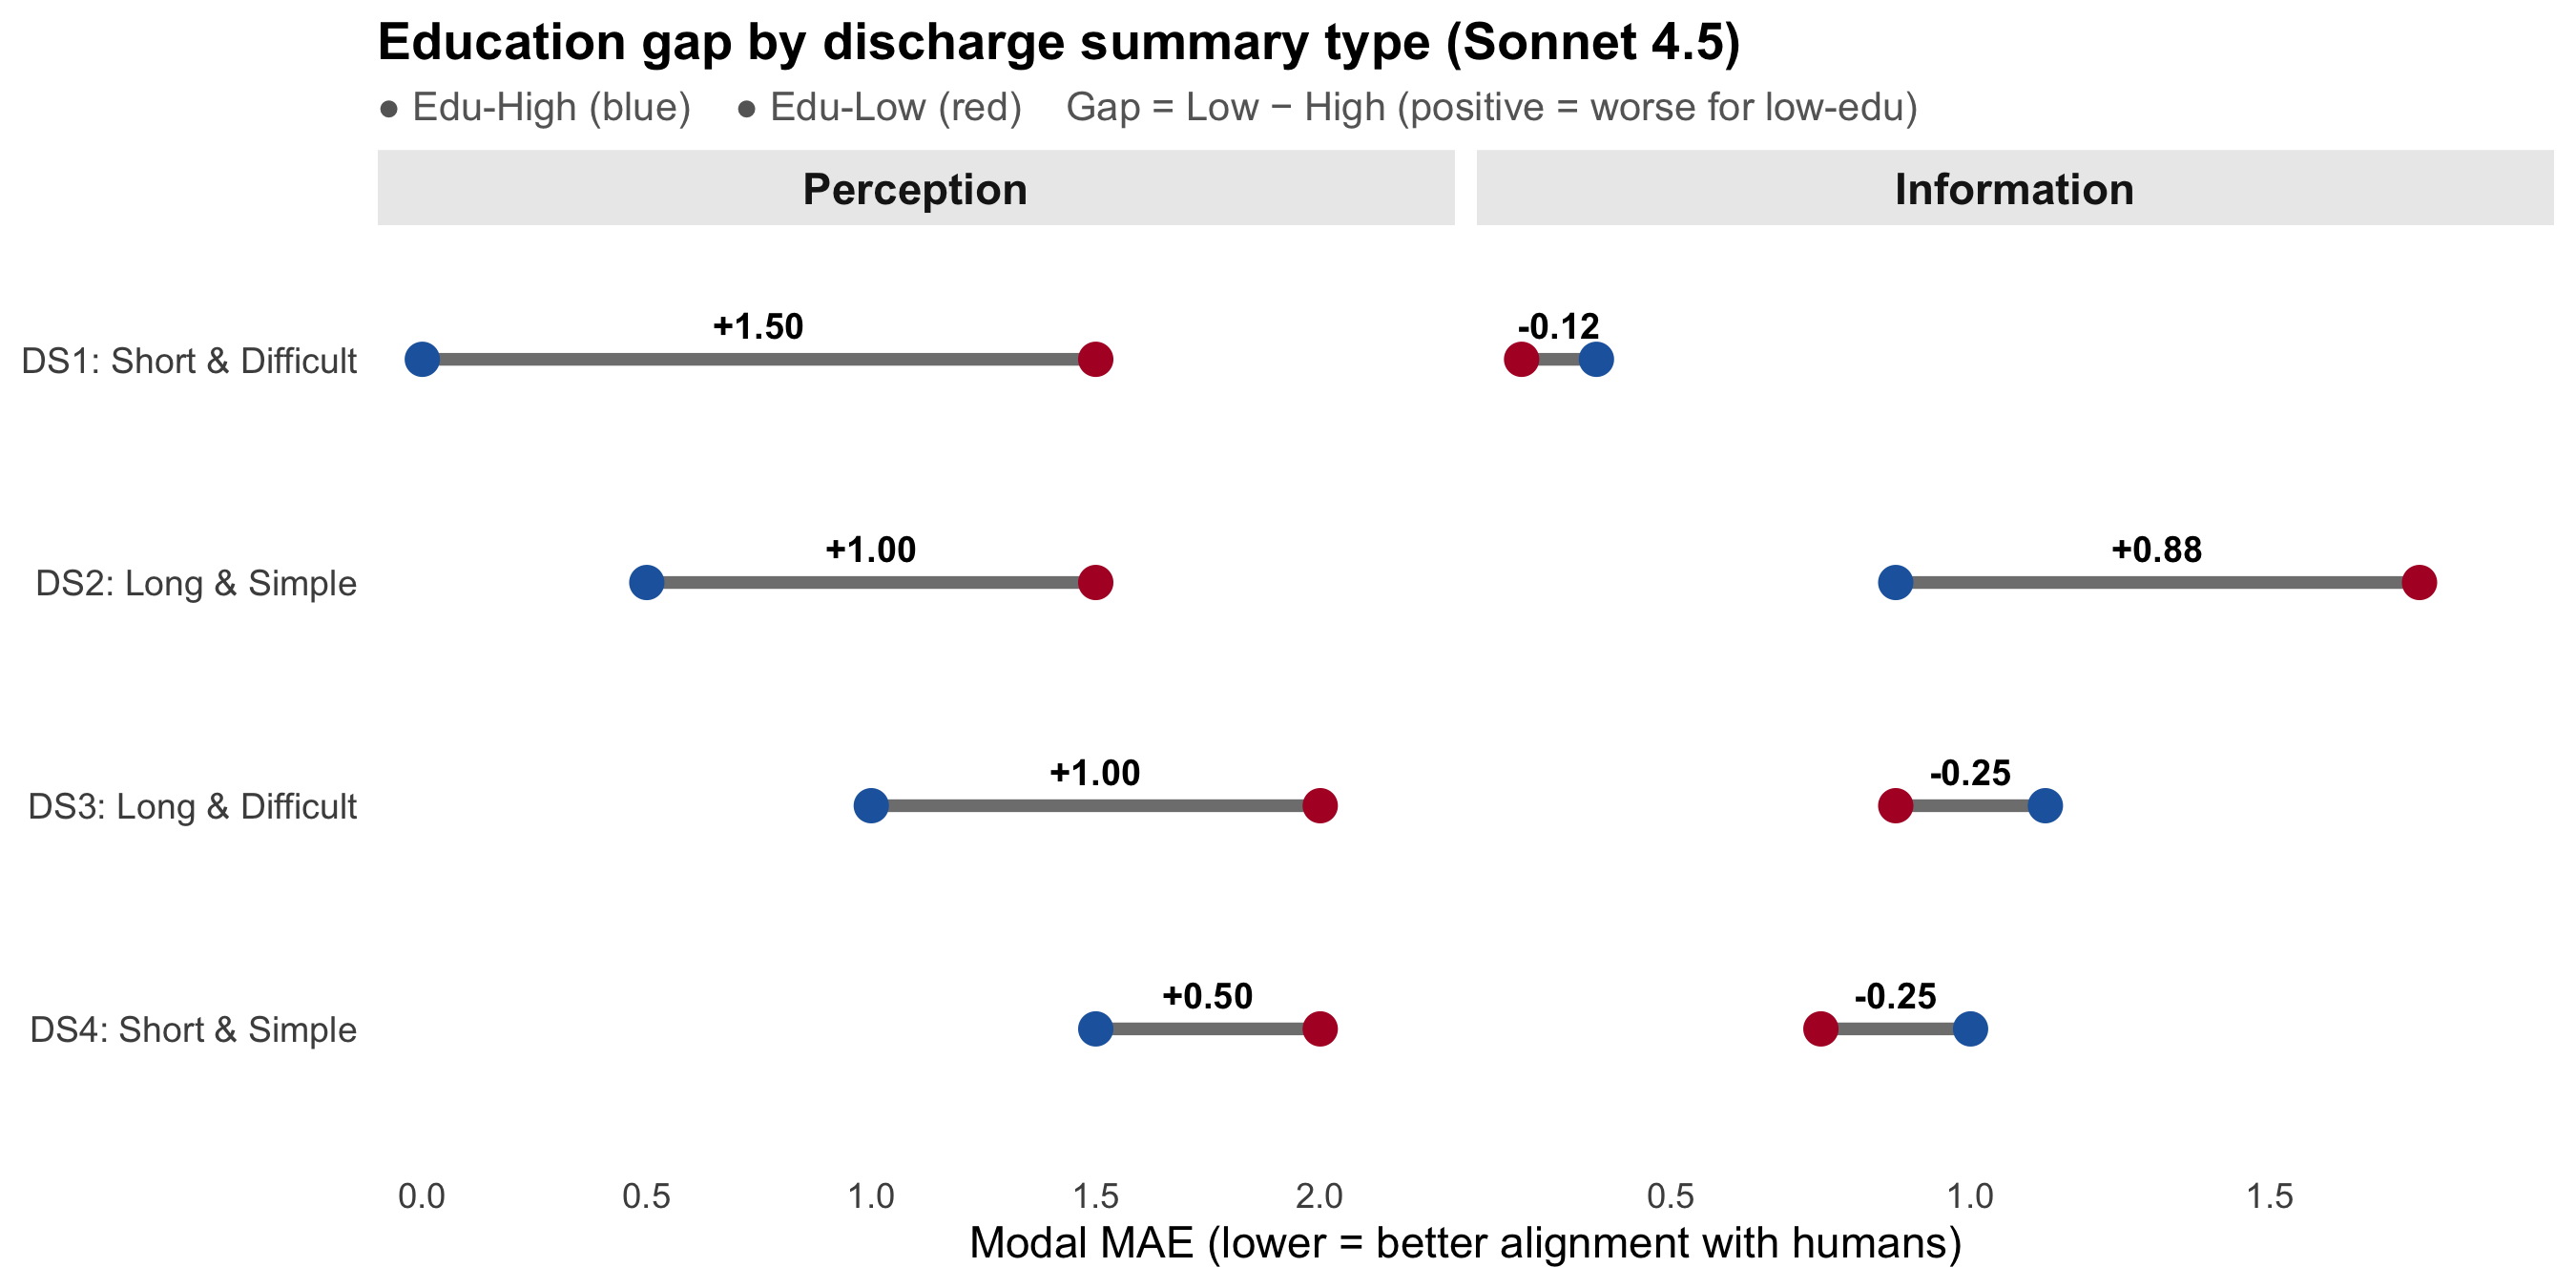
\includegraphics[width=\textwidth]{ds_edu_dumbbell.png}
\caption{Education gap by discharge summary type for Sonnet~4.5. Each row
represents one DS type. Blue dots indicate the modal MAE for the Edu-High
subgroup; red dots indicate Edu-Low. The connecting line length corresponds
to the education gap ($\Delta$\,$=$\,Low$-$High); annotated values above
each line. Left panel: perception-based questions (Q1, Q10); right panel:
information-based questions (Q2--Q9). DS1 (Short \& Difficult) exhibited the
largest perception gap (+1.50).}
\label{fig:ds-edu-dumbbell}
\end{figure}

% ---------- Figure 2: Perception stacked bars ----------
\begin{figure}[htbp]
\centering
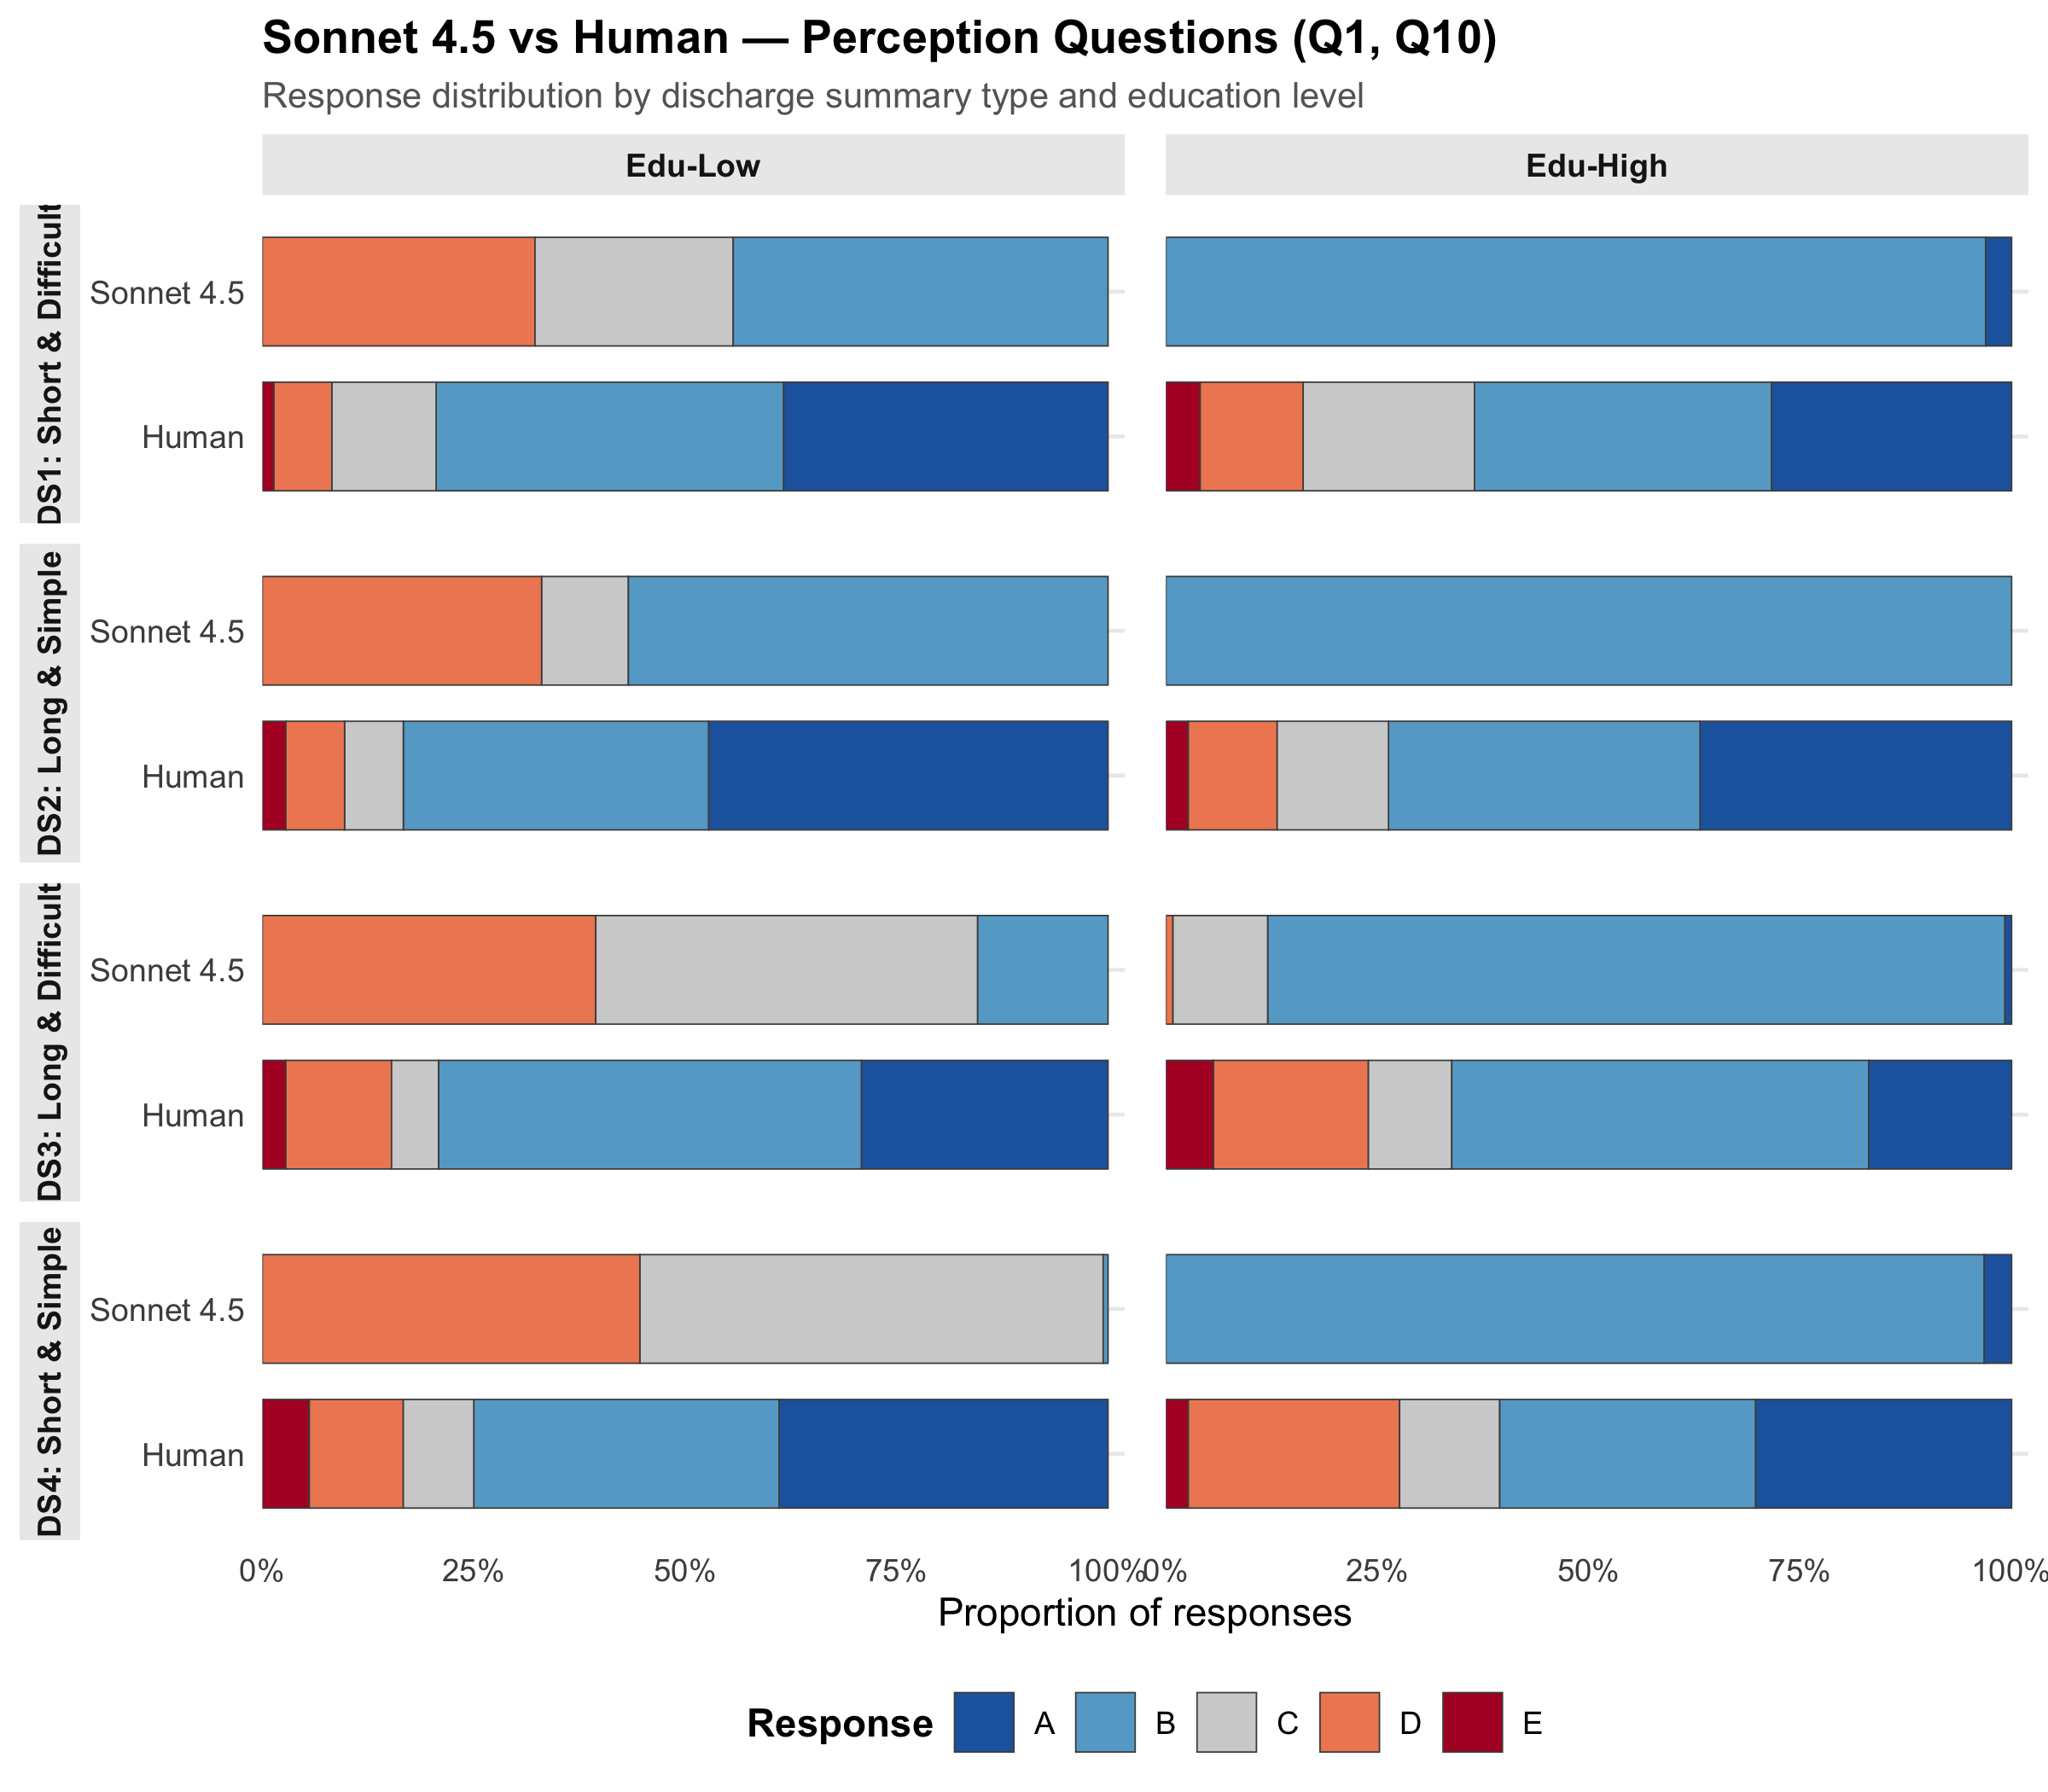
\includegraphics[width=\textwidth]{ds_edu_perception_dist.png}
\caption{Response distributions for perception-based questions (Q1, Q10),
comparing Sonnet~4.5 against human respondents. Rows: 4 discharge summary
types; columns: Edu-Low vs Edu-High. Each horizontal stacked bar shows the
proportion of responses from A (dark blue, most positive) through E (dark
red, most negative). For DS1 Edu-Low, the human distribution concentrates
on A--B while Sonnet~4.5 shifts mass toward C--D, illustrating the
model's tendency to assume lower clarity and confidence for low-education
personas.}
\label{fig:ds-edu-perception-dist}
\end{figure}

% ---------- Figure 3: Information stacked bars ----------
\begin{figure}[htbp]
\centering
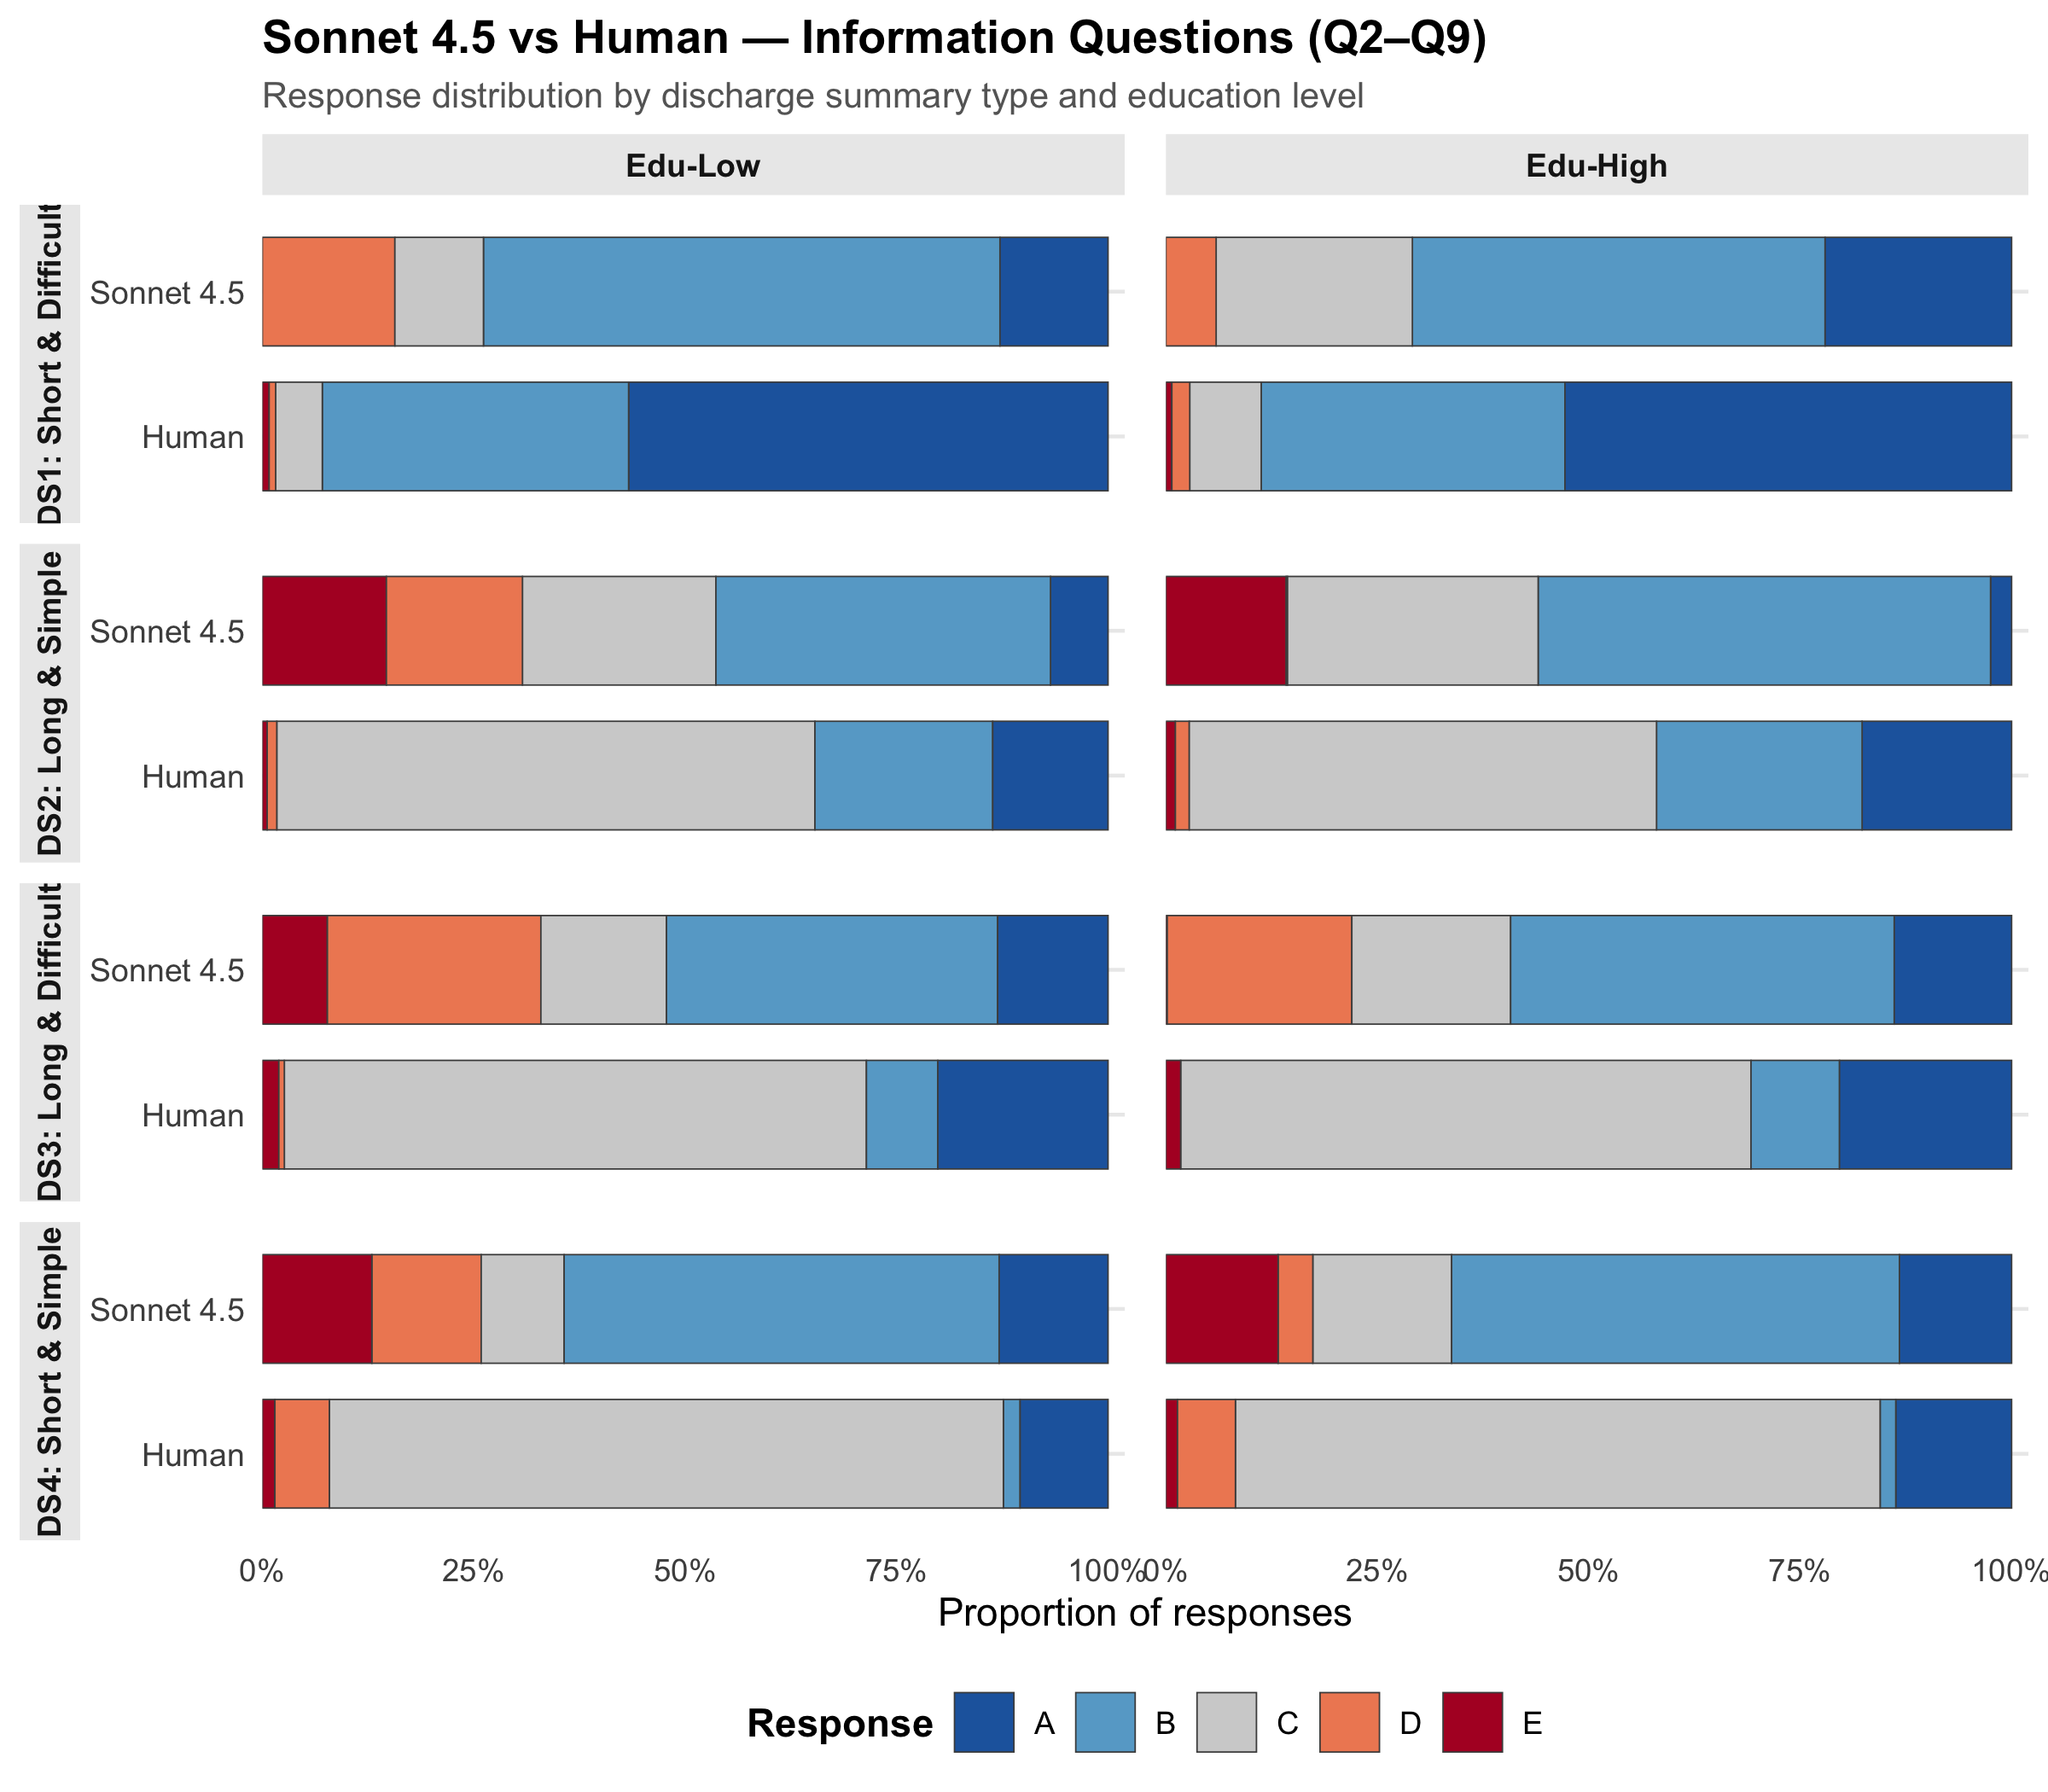
\includegraphics[width=\textwidth]{ds_edu_information_dist.png}
\caption{Response distributions for information-based questions (Q2--Q9),
comparing Sonnet~4.5 against human respondents. Same layout as
Figure~\ref{fig:ds-edu-perception-dist}. The reversed gap on DS1
(Short \& Difficult) is visible: Edu-Low distributions more closely
resemble the human pattern than Edu-High on this discharge summary type.}
\label{fig:ds-edu-information-dist}
\end{figure}


\subsection{Sex Gap by Discharge Summary Type}

To assess whether the sex gap exhibited a comparable DS-dependent pattern, we
computed per-DS sex gaps (Male$-$Female) for all 4 models on perception modal MAE
(Table~\ref{tab:ds-sex-gap-perc}).

% ---------- Table 8: Per-DS Sex Gap (all models, Perception MAE) ----------
\begin{table}[htbp]
\centering
\scriptsize
\setlength{\tabcolsep}{5pt}
\caption{Per-DS sex gap on perception modal MAE (Male$-$Female) for all 4 models.
Positive values indicate worse alignment for the male subgroup. Bold marks the
largest absolute gap per model.}
\label{tab:ds-sex-gap-perc}
\begin{tabular}{lrrrr}
\toprule
\textbf{DS Type} & \textbf{Sonnet 4.5} & \textbf{Opus 4.6} & \textbf{GPT-5.2} & \textbf{GPT-4.1} \\
\midrule
DS1: Short \& Difficult & +0.50 &  0.00 & +0.50 & +0.50 \\
DS2: Long \& Simple     &  0.00 &  0.00 &  0.00 &  0.00 \\
DS3: Long \& Difficult  & +0.50 & $-$0.50 & \textbf{+1.50} & \textbf{+1.00} \\
DS4: Short \& Simple    & $-$0.50 & \textbf{+0.50} & $-$0.50 & \textbf{+1.00} \\
\midrule
Overall                 & +0.12 &  0.00 & +0.38 & +0.62 \\
\bottomrule
\end{tabular}
\end{table}

Unlike the education gap, the sex gap did not exhibit a consistent DS-dependent
pattern across models. Three observations are noteworthy:

\begin{enumerate}\itemsep2pt
\item \textbf{No model showed a unidirectional sex gap across all DS types.}
  Every model had at least one DS where the gap was zero or favored the opposite
  sex. By contrast, Sonnet~4.5's education gap was positive (Edu-Low worse)
  across all 4 DS types (Table~\ref{tab:ds-edu-gap}). This directional
  inconsistency indicates that sex-based differences in persona alignment are
  driven by question-level mode flips rather than a systematic bias.

\item \textbf{Isolated large gaps appeared for GPT-5.2 and GPT-4.1 on specific
  DS types.} GPT-5.2 exhibited a sex gap of +1.50 on DS3 (Long \& Difficult),
  the single largest sex-related cell in the analysis, and GPT-4.1 showed +1.00
  on both DS3 and DS4. However, these were offset by zero or reversed gaps on
  other DS types, producing moderate overall gaps (+0.38 and +0.62, respectively).

\item \textbf{Opus~4.6 remained the most equitable model.} Its perception sex gap
  never exceeded $|$0.50$|$ on any DS type and averaged 0.00 overall,
  consistent with its overall equity advantage reported in
  Table~\ref{tab:sex-gap}.
\end{enumerate}

The EAD sex gaps were uniformly small across all models and DS types
(all $|$$\Delta$$|$$\le$0.28), further confirming that the perception modal MAE
differences reflected mode-switching sensitivity rather than broad distributional
mismatch. These results suggest that discharge summary characteristics modulate
the education gap far more systematically than the sex gap, making education
level the primary equity concern for LLM-based persona simulation in
patient-centric communication.


\subsection{Per-Question Misalignment Analysis: Sonnet 4.5 on Information Questions}

Sonnet~4.5 exhibited the worst alignment on information-based questions
across all metrics (modal MAE\,$=$\,0.90; EAD\,$=$\,0.92; K-S $D$\,$=$\,0.221).
To understand the mechanisms driving this misalignment, we examined all 32
information questions (4 DS $\times$ 8 questions) at the per-question level,
comparing Sonnet~4.5's pooled modal response against the human pooled modal
response. Table~\ref{tab:misalignment-summary} summarizes the degree of
misalignment; Table~\ref{tab:misalignment-detail} presents the 7 worst-aligned
questions with full response distributions. For multi-select questions
(check-all-that-apply), each chosen option contributes one vote so the
reported distributions reflect overall option-selection prevalence.

% ---------- Table 9: Misalignment Summary ----------
\begin{table}[htbp]
\centering
\scriptsize
\setlength{\tabcolsep}{5pt}
\caption{Per-question misalignment summary for Sonnet~4.5 on information-based
questions ($n$=32). Ordinal distance between LLM modal response and human
modal response.}
\label{tab:misalignment-summary}
\begin{tabular}{lrr}
\toprule
\textbf{Modal Distance} & \textbf{Count} & \textbf{\%} \\
\midrule
0 (perfect match)       & 11 & 34.4 \\
1 (off by one)          & 14 & 43.8 \\
2+ (off by two or more) &  7 & 21.9 \\
\bottomrule
\end{tabular}
\end{table}

% ---------- Table 10: Worst Misaligned Questions ----------
\begin{table}[htbp]
\centering
\scriptsize
\setlength{\tabcolsep}{3pt}
\caption{Seven worst-aligned information questions for Sonnet~4.5 (modal
distance $\ge$2). Response distributions shown as percentages of each
option chosen. Human $n$$\approx$75 per question; LLM
$n$$\approx$7{,}680 pooled across 10 iterations and all personas.}
\label{tab:misalignment-detail}
\begin{tabular}{llcccp{3cm}p{3.5cm}}
\toprule
\textbf{Question} & \textbf{Topic}
& \textbf{Hum} & \textbf{LLM} & \textbf{Dist}
& \textbf{Human Distribution} & \textbf{LLM Distribution} \\
\midrule
DS2-Q6 & When to call doctor & A & E & \textbf{4}
& A:34\% B:33\% D:32\% & E:100\% \\
DS1-Q9 & Discharge plan coverage & D & B & 2
& A:19\% C:22\% D:22\% E:20\% & B:71\% D:29\% \\
DS2-Q7 & Activities prohibited & B & D & 2
& B:41\% C:21\% D:37\% & B:40\% C:11\% D:48\% \\
DS2-Q9 & Discharge plan coverage & A & C & 2
& A:30\% B:22\% D:16\% E:11\% G:8\% & C:40\% D:37\% E:17\% B:6\% \\
DS3-Q5 & Test results identified & C & A & 2
& A:40\% B:10\% C:50\% & A:100\% \\
DS3-Q9 & Discharge plan coverage & C & E & 2
& A:20\% B:14\% C:24\% E:21\% & E:61\% C:39\% \\
DS4-Q5 & Test results identified & C & A & 2
& A:11\% B:9\% C:80\% & A:100\% \\
\bottomrule
\end{tabular}
\end{table}

% ---------- Figure 4: Misalignment stacked bars ----------
\begin{figure}[htbp]
\centering
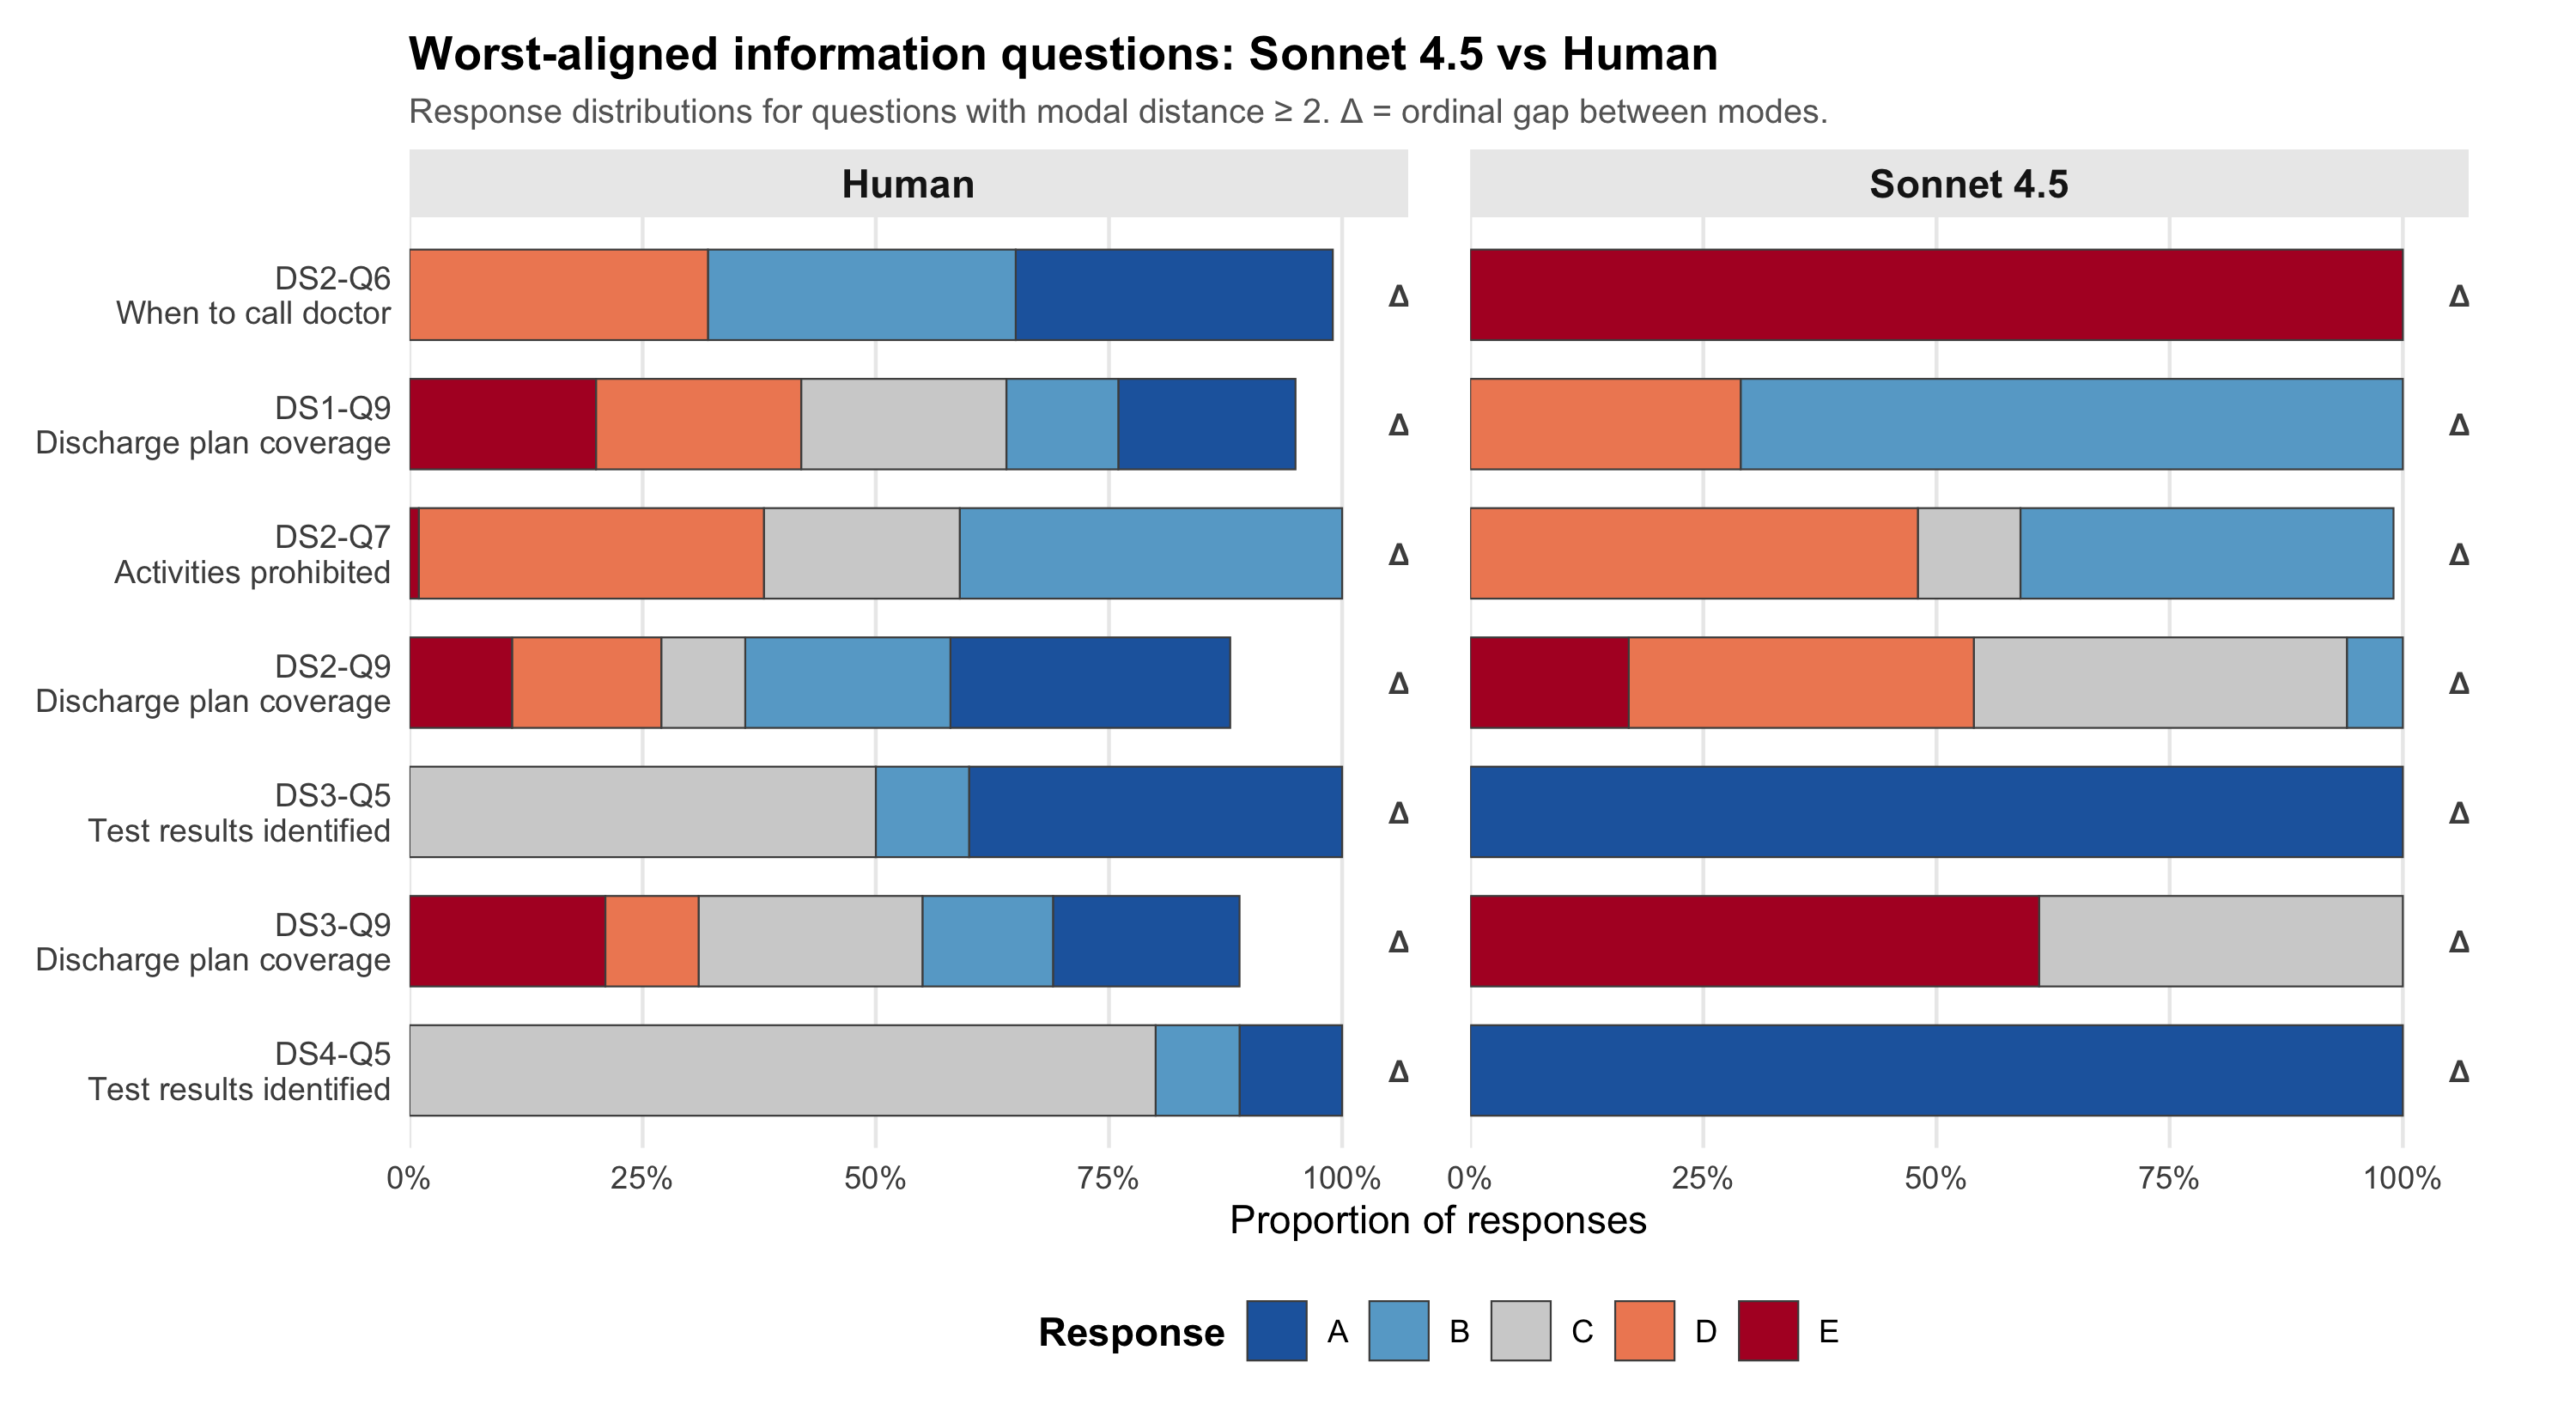
\includegraphics[width=\textwidth]{misalignment_worst_questions.png}
\caption{Response distributions for the 7 worst-aligned information questions
(modal distance $\ge$2) comparing Sonnet~4.5 against human respondents.
Left panel: human distributions; right panel: LLM distributions. Colors
encode ordinal responses from A (dark blue, most positive) through E (dark
red, most negative). The $\Delta$ annotation indicates the ordinal gap
between modal responses. DS2-Q6 (``when to call the doctor'') shows the
largest gap ($\Delta$=4): the model collapses on E (``all of the above'')
while humans select individual symptoms (A:34\%, B:33\%, D:32\%). Discharge
plan coverage (Q9) and test results identification (Q5) account for the
remaining six $\Delta$$\ge$2 gaps.}
\label{fig:misalignment-worst}
\end{figure}

Four distinct misalignment patterns emerged:

\subsubsection{Pattern 1: Systematic ``Identified'' Bias on Factual Extraction (Q2--Q4)}

The most pervasive pattern affected the factual-extraction questions across
DS2--DS4. On items asking whether specific clinical information (diagnosis,
cause, tests) could be identified in the discharge summary, Sonnet~4.5
selected option B (``Yes, identified'') with near-100\% probability, while
human respondents predominantly selected option C (``Not provided'') with
54--87\% frequency on the same questions. This pattern reveals a fundamental
information-extraction bias: the model assumes that clinical content is
readily identifiable in the discharge summary, whereas human
patients---regardless of education level---frequently report that the
information was not clearly provided. This ``identification optimism''
likely stems from the model's ability to extract information from text that
patients find ambiguous or inaccessible.

\subsubsection{Pattern 2: ``When-to-call-the-doctor'' Collapse (DS2-Q6)}

The single largest gap (modal distance $=$ 4) occurred on DS2-Q6,
which asks which symptoms should prompt a call to the doctor. The
model placed 100\% of its mass on option E (``All of the above''),
whereas humans almost never picked the catch-all and instead distributed
their selections across individual symptoms (A: Fever\,$>$\,101 = 34\%;
B: Chest Pain = 33\%; D: Shortness of breath = 32\%). The model treats
the multi-select question as if the safest answer is to flag every
symptom; human respondents, by contrast, select the specific symptoms
that the discharge summary actually warns about. This is the only
question in the entire information block with a $\Delta$\,$\ge$\,3 gap.

\subsubsection{Pattern 3: Test Results Reversal (Q5)}

On test results identification (Q5), the model exhibited a directional
reversal across discharge summaries. On DS3 and DS4, where 50--80\% of
humans selected C (``not provided''), the model placed 100\% of its mass on
A (``identified''). On DS1 the human and model modes coincide on C (humans
76\%, model 92\%). The model thus over-claims that test results are
present in the long, dense discharge summaries (DS3, DS4) while patients
on the same documents report the opposite.

\subsubsection{Pattern 4: Multi-Select ``Discharge Plan Coverage'' (Q9 across DSes)}

The Q9 item (``which of the following does your discharge plan cover?'')
is a check-all-that-apply question with 7 options (medication schedule,
follow-up, symptoms, diet, activity, other, none). Three of the four DSes
(DS1, DS2, DS3) yielded a $\Delta$\,$=$\,2 gap: the model concentrates on
one or two components (e.g., DS1: B+D = 100\%; DS3: C+E = 100\%), while
humans report broader and more varied coverage that spans 4--5 options.
The model treats this question as single-best-answer rather than recognizing
its check-all-that-apply nature, producing systematically narrower coverage
profiles than the human-reported ones.

\subsubsection{Summary}

Eleven of 32 information questions (34\%) achieved perfect modal alignment;
the dominant failure mode for the remaining 21 was a systematic
identification-optimism bias on factual-extraction questions (Q2--Q5),
where Sonnet~4.5 assumed clinical information was identifiable when
patients reported it was not. The single most extreme gap occurred on a
``when-to-call-the-doctor'' multi-select question, where the model
collapsed onto the catch-all ``all of the above'' rather than the
specific symptoms emphasized in the discharge summary, and an analogous
single-best-answer collapse degraded the multi-select ``discharge plan
coverage'' question (Q9) across three of the four DSes. These results
suggest that the model's superior text comprehension paradoxically
undermines its ability to simulate patients who may lack the medical
literacy to locate the same information, and that it does not naturally
distinguish multi-select questions from single-choice ones.
